To prove the functional correctness of real graph-manipulating
algorithms, we provide spatial predicate of graphs as a shape
description about heaps. As a matter of fact, we defined a much more
general spatial predicate ``$\bigstar$'' to indicate a collection of
standard points-to predicates chained by $\scon$ in separation
logic. The spatial graph predicate is just a special case in terms of
$\bigstar$.

\subsection{Infrastructure}
To formalize spatial graphs and related lemmas, we need a way to
represent spatial predicate first, in other words, a mechanized
library of separation logic. We adopt a layered style to get things
done: Our spatial graph definition is build on a separation logic
layer which are composed by atomic notations ($\scon$, $\ocon$, $|->$,
$\p{precise}$, etc.) and related properties as axioms. Under the logic
layer are sound models of the logic.

\begin{figure}[htbp]
\centering
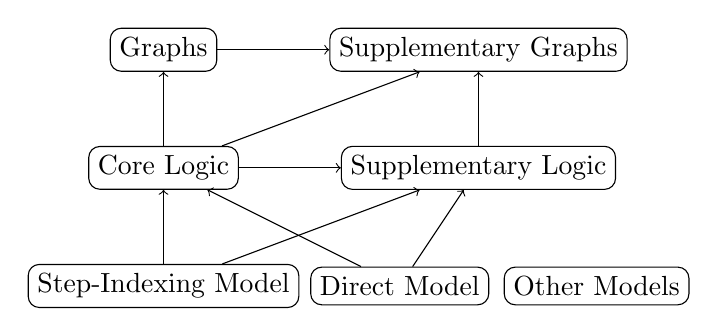
\begin{tikzpicture}
\tikzstyle{every node}=[shape=rectangle, rounded corners=4pt, draw]
\node (SM) at (-3, 0) {Step-Indexing Model};
\node (DM) at (0, 0) {Direct Model};
\node (OM) at (2.5, 0) {Other Models};
\node (CL) at (-3, 1.5) {Core Logic};
\node (SL) at (1, 1.5) {Supplementary Logic};
\node (G) at (-3, 3) {Graphs};
\node (SG) at (1, 3) {Supplementary Graphs};
\draw [->] (CL) to (G);
\draw [->] (G) to (SG);
\draw [->] (CL) to (SG);
\draw [->] (SL) to (SG);
\draw [->] (CL) to (SL);
\draw [->] (SM) to (CL);
\draw [->] (SM) to (SL);
\draw [->] (DM) to (CL);
\draw [->] (DM) to (SL);
%% \draw [->] (OM) to (CL);
%% \draw [->] (OM) to (SL);
\end{tikzpicture}
\caption{Infrastructure of spatial graph library}
\end{figure}

%% 2.3. \texttt{sSpatialGraph\_Graph\_Bi} defined in "\texttt{spatial\_graph\_bi.v}" is the premise type class for defining how a BiMaFin graph is stored in memory.

%% 2.5. Heap-Model-Direct instances are broken now. They are not hard to get fixed. Previous proofs are in "\texttt{spatial\_graph\_HMD.v}".

\subsection{Traditional fixpoints fail}\label{sec:fixpointfail}

As shown in (\ref{eqn:bigraphintrofoldunfold}) of Section
\ref{sec:orientation}, Hobor and Villard\cite{hobor:ramification}
defined the separation logic graph predicate
$\mathsf{graph}(x,\gamma)$ in direct analogy to the standard
separation logic definition of a tree. Note that the two-neighborhood
means $\gamma$ is a BiGraph. However, it is peculiarly challenging in
rigorously formalizing $\p{graph}$.

%* Showing that neither traditional fixpoint method works

Recursive/inductive predicates are ubiquitous in separation logic---so
much so that when a person writes the definition of a predicate as $P$
``$\defeq$'' $\ldots P \ldots$ no one raises an eyebrow, despite the
dangers of circularity in mathematics. Indeed, 95\% of the time there
is no danger thanks to the magic of the Knaster/Tarski fixpoint
$\mu_{\mathsf{T}}$ \cite{tarski:fixpoint}. Formally what is going on
is instead of defining $P$ directly, one defines a functional $F_P
\defeq \lambda P.~ \ldots P \ldots$ and then defines $P$ itself as $P
\defeq \mu_{\mathsf{T}} \, F_P$.  Assuming (as one typically does
without comment) that $F_P$ is \emph{covariant}, i.e. $(P \vdash Q)
\Rightarrow (F \, P \vdash F \, Q)$, one then enjoys the fixpoint
equation $P \Leftrightarrow \ldots P \ldots$, formally justifying
typically written pseudodefinition (``$\defeq$'').

Appel and McAllester developed an additional fixpoint
$\mu_{\mathsf{R}}$ \cite{appel:fixpoint} whose \cite{appel:vmm}
mechanically verified its soundness. People can still define recursive
predicate $P$ through $F_p$ and $\mu_{\mathsf{R}}$, but this time the
$F_p$ needs to be \emph{contractive}. Informally, a contractive
function is one such that if $\tau$ is approximately equal to
$\sigma$, then $F_p(\tau)$ is more accurately equal to
$F_p(\sigma)$. The approximate equality is achieved by a data type as
a sequence of accurate approximations taken successively. This idea is
called step-indexing.

We attempted to formulate $\mathtt{graph}$ through fixed-point
functions $\mu_{\mathsf{T}}$ and $\mu_{\mathsf{R}}$. The contractive
functor $\mathtt{graphF}$ is defined as follows:
\[\label{eqn:graphFcotr}
  \begin{split}
  & \mathtt{graphF}(Q, x, \gamma)\defeq (x = 0 \wedge \mathtt{emp})
    \vee \\ & \exists d,l,r . \gamma(x)=(d,l,r) \wedge x \mapsto
    d,l,r\, \ocon \triangleright Q(l, \gamma) \ocon \triangleright
    Q(r, \gamma)
  \end{split}
\]
where $\triangleright$ is is the ``later'' operator which implements
the machinery of step-indexing. Note that $\mathtt{graphF}$ is a
normal predicate without recursion. $\mathtt{graph}$ is defined as
$\mu_{\mathsf{R}}\,\mathtt{graphF}$. One advantage of this definition
of $\mathtt{graph}$ is that proof by induction is possible because the
step-index can be seen as the inductive number. Unfortunately
$\mathtt{graph}$ is not \emph{precise} under this definition. For any
spatial predicate $P$, $\text{precise}(P)$ means whenever $P$ is
satisfied on a sub-state, that sub-state must be unique. Being precise
is a crucial requirement of $\mathtt{graph}$ for key theorems in our
framework. Further-more, it can be proved that for any predicate $P$,
$\triangleright P$ is not precise. So this defintion is abandoned.

Similarly we can define a covariant functor $\mathtt{graphQ}$ as
follows:
\[\label{eqn:graphFco}
  \begin{split}
  & \mathtt{graphQ}(Q, x, \gamma)\defeq (x = 0 \wedge
  \mathtt{emp}) \vee \\ & \exists d,l,r . \gamma(x)=(d,l,r) \wedge  x
  \mapsto d,l,r\, \ocon Q(l, \gamma) \ocon Q(r, \gamma)
  \end{split}
\]
The only difference between $\mathtt{graphQ}$ and $\mathtt{graphF}$ is
that $\mathtt{graphQ}$ does not have the $\triangleright$
operator. With this definition $\mathtt{graph}$ can be defined as
$\mu_{\mathsf{T}}\,\mathtt{graphQ}$. Again we need to prove the
preciseness of $\mathtt{graph}$. Since there is no induction principle
for this definition, we tried to prove it through the following lemma:
\begin{equation}\label{eqn:graph_iter}
\mathtt{graph}(x, \gamma) \dashv\vdash
\underset{v\in\mathit{reach}(\gamma, x)}{\bigstar} v\mapsto\gamma(v)
\end{equation}
where $\mathit{reach}(\gamma, x)$ is the set of nodes reachable from
$x$ in $\gamma$ and the definition of $\bigstar$ over a set and a
predicate $p$ is
\begin{equation*}
  \underset{\{a_1, a_2,\dots,a_n\}}{\bigstar}p \defeq p(a_1) \scon
  p(a_2) \scon \dots \scon p(a_n).
\end{equation*}
The preciseness of $\mathtt{graph}$ is a natural corollary of the
lemma above because for any $v$, $v\mapsto\gamma(v)$ is
precise. Unfortunately that lemma does not hold even for a
self-referencing single node graph because: every time the expanding
of $\mathtt{graph}(x,\gamma)$ leads to itself. So this definition is
abandoned too.

Although the traditional fixpoints fail for spatial graphs, it is
worth mentioning that the traditional fixpoints work for trees, lists,
dags and etc, as long as they do not contain cycles.

\subsection{The iterated separating conjunction}\
The two failures of fixpoint method above force us to turn to another
direction. Inspired by lemma \ref{eqn:graph_iter}, we defined the
$\mathtt{graph}$ as follows:
\begin{equation}\label{eqn:iter_def}
  \mathtt{graph}(x, \gamma)\defeq\underset{v\in\mathit{reach}(\gamma, x)}{\bigstar} v\mapsto\gamma(v)
\end{equation}

This non-recursive predicate says that a graph whose root is $x$ is a
list of reachable nodes from $x$ separated by $\scon$.

\label{sec:foldunfold} From this definition we can prove the unfold lemma:
\begin{equation*}
  \begin{split}
  & \mathtt{graph}(x, \gamma) \Leftrightarrow \exists d,l,r
    . \gamma(x)=(d,l,r) \wedge \\ & x \mapsto d,l,r\, \ocon
    \mathtt{graph}(l, \gamma) \ocon \mathtt{graph}(r, \gamma)
  \end{split}
\end{equation*}

One useful property in proving the unfold lemma is \emph{joinable}. A
predicate $p$ is joinable iff for any $x\neq y$, $p(x)$ and $p(y)$ are
in disjointed heap, which means we can write $p(x) * p(y)$.

One benefit of the definition in (\ref{eqn:iter_def}) is that the pure
mathematical graph $\gamma$ in $\mathtt{graph}$ is not necessarily a
BiGraph. (\ref{eqn:iter_def}) can represent a general graph with
variant number of neighors as long as extending the definition of
$\gamma(x)$ to data mapped by the label function and every neighbor of
node $x$.

Moreover, it turns out that the $\bigstar$ notation is a more useful
and fundamental concept than $\mathtt{graph}$. There are two parts of
the $\bigstar$ in (\ref{eqn:iter_def}): one is the predicate $\mapsto$
and the other is the node set which the $\mapsto$ iterates on. They
both bind to $\gamma$ in (\ref{eqn:iter_def}) for $\p{graph}(x,
\gamma)$, which is a special case. In section \ref{sec:applicable}, we
will see the specification of a spanning tree algorithm which uses
$\bigstar$ directly instead of $\p{graph}$ because in that
specification, the predicate $\mapsto$ and the node set bind to
different mathematical graphs. Furthermore, we generalize the
ramification rules for $\p{graph}$ in \cite{hobor:ramification}, which
uses $\bigstar$ so as to be applied in all verification examples.

%% 1.2. \texttt{Iter\_sepcon} and \texttt{pred\_sepcon} are defined. And related ramification rules are proved.
%% 1.3. The most general graph-spatial-predicate \texttt{vertices\_at} are defined (for all possible styles of graphs). Related ramification rules are proved. Graph and graphs are defined as special cases of vertices at.

%% 2. A minor implementation trick. There are many tactics defined in \texttt{msl\_ext/ramify\_tactics.v}, which can manipulate low level heaps efficiently.

%% * Separating the material into the general vs. tool-specific part.  Measurements of etc.
